\documentclass{article}
\usepackage{hyperref}
\usepackage{graphicx}
\usepackage{float}
\usepackage{amsmath}

\title{Computer Vision HW10 Report}
\author{B01902044 Steven Lin}
\date{2015-12-16}

\newcommand{\code}[1]{\texttt{#1}}

\begin{document}

\pagenumbering{gobble}
\maketitle
\newpage

\pagenumbering{arabic}

\tableofcontents
\newpage

% ---------- 1st section: source code ---------- %
\section{Source Code}
This part of the report will go through some important snippets of my source code. For source code file, please check out the \code{hw10.py} file in the directory submitted.

\subsection{Principle Code Sneak Peek}
First, we will take a look at the overall structure of my code. And furthermore we will have some brief explanation for the implementation of the operators with different masks.

\subsubsection{Functions Overview}
In this homework, we are asked to implement 5 different kinds of zero-crossing edge detection methods. And there are 4 functions that I've created for those methods. \\
The following snapshot includes the signature of those 4 functions.\\
\begin{figure}[H]
  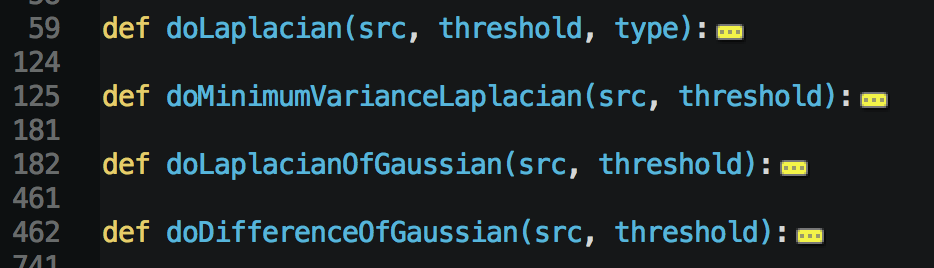
\includegraphics[width=\linewidth]{img/functions_overview.png}
  \caption{Essential Functions Overview}
  \label{fig:functions_overview}
\end{figure}
All of the functions above take these parameters: \code{src} and \code{threshold}, which respectively stands for source image (input image) and the threshold for this method. And all the functions, if no error occurs, return a new image which is properly processed image. \\
The function \code{doLaplacian();} takes an additional parameter: \code{type} due to the fact that we have 2 different masks for Laplacian method. And the \code{type} parameter should be either \code{1} or \code{2}; otherwise, the function returns the source image \code{src} without any processing.

\subsubsection{Masks to be used}
There are 5 different masks (kernels), and they result in 5 different images in the end. \\
The masks that I have utilized in my code (in \code{hw10.py}) are shown in the following figure.
\begin{figure}[H]
  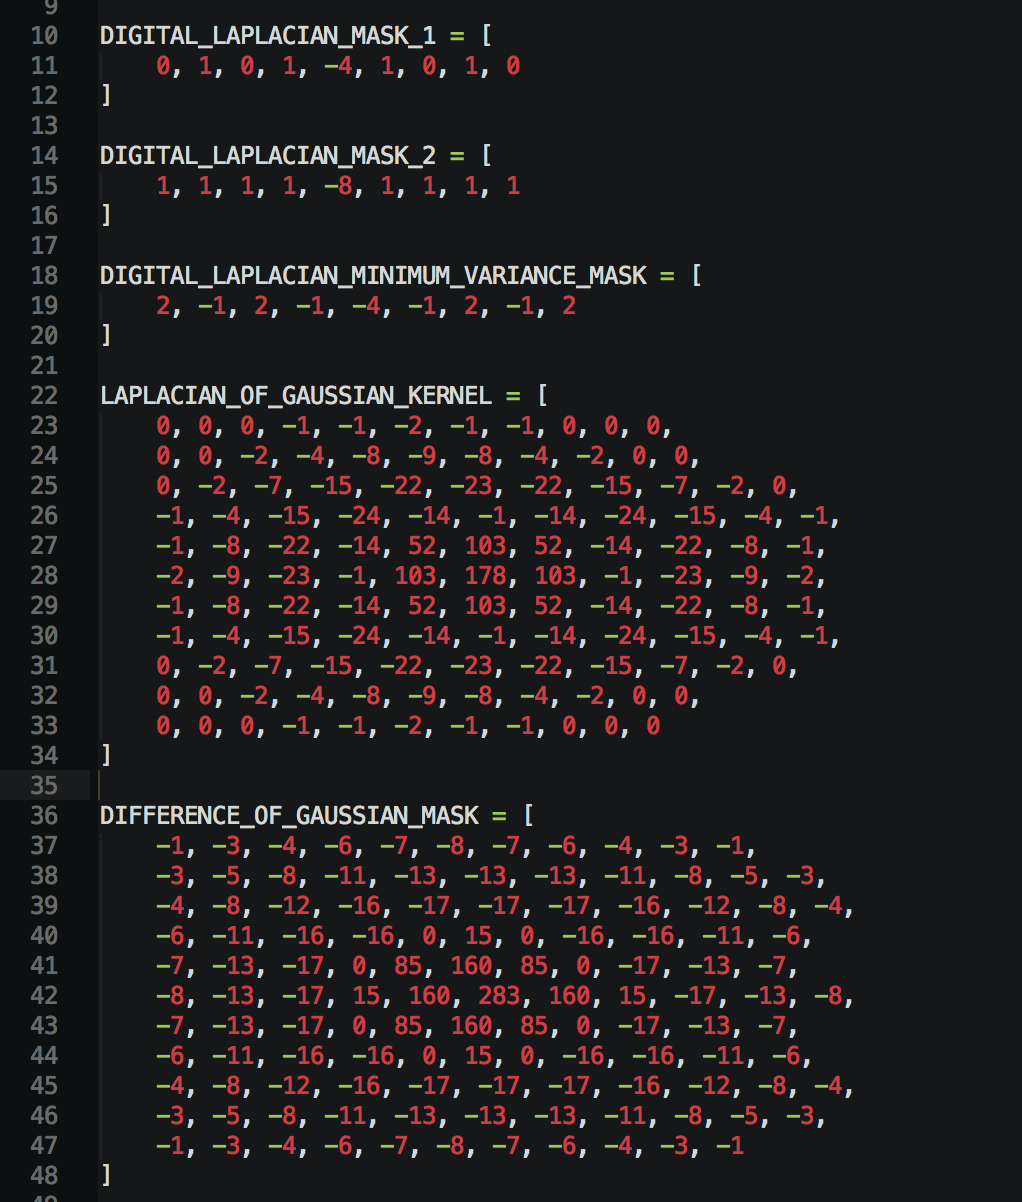
\includegraphics[width=\linewidth]{img/masks.png}
  \caption{Masks to be used in this homework}
  \label{fig:masks}
\end{figure}
\paragraph{DIGITAL\_LAPLACIAN\_MASK\_1} the mask for Laplacian type 1.
\paragraph{DIGITAL\_LAPLACIAN\_MASK\_2} the mask for Laplacian type 2.
\paragraph{DIGITAL\_LAPLACIAN\_MINIMUM\_VARIANCE\_MASK} the mask for Minimum Variance Laplacian.
\paragraph{LAPLACIAN\_OF\_GAUSSIAN\_KERNEL} the kernel for Laplace of Gaussian.
\paragraph{DIFFERENCE\_OF\_GAUSSIAN\_MASK} the mask for Difference of Gaussian.
\paragraph{BBB mask} for BBB.

\subsection{Parameters (Threshold)}
Here is the list of thresholds I used for each of the resulted image.
\begin{description}
  \item[Laplacian Mask Type 1] \hfill \\
  my threshold = 15
  \item[Laplacian Mask Type 2] \hfill \\
  my threshold = 15
  \item[Minimum Variance Laplacian] \hfill \\
  my threshold = 20
  \item[Laplace of Gaussian] \hfill \\
  my threshold = 3000
  \item[Difference of Gaussian] \hfill \\
  my threshold = 1
\end{description}

% ---------- 2nd section: results ---------- %
\section{Results}
All the resulted images are properly saved and submitted along with this report document. You may go check them out if you'd like to.

\subsection{Laplacian Mask Type 1}
\begin{figure}[H]
  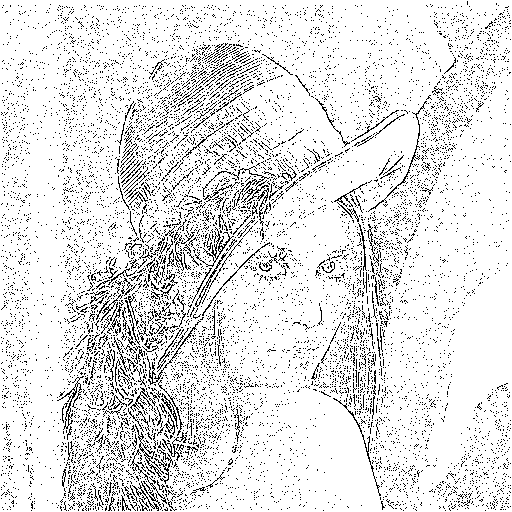
\includegraphics[width=\linewidth]{img/laplacian_1.png}
  \caption{Laplacian type 1 with threshold=15}
  \label{fig:laplacian_1}
\end{figure}

\subsection{Laplacian Mask Type 2}
\begin{figure}[H]
  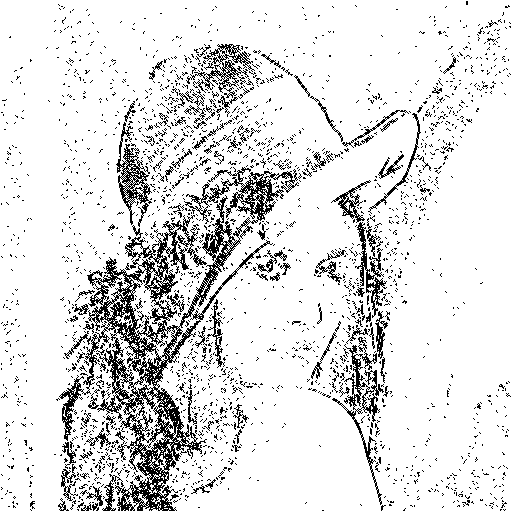
\includegraphics[width=\linewidth]{img/laplacian_2.png}
  \caption{Laplacian type 2 with threshold=15}
  \label{fig:laplacian_2}
\end{figure}

\subsection{Minimum Variance Laplacian}
\begin{figure}[H]
  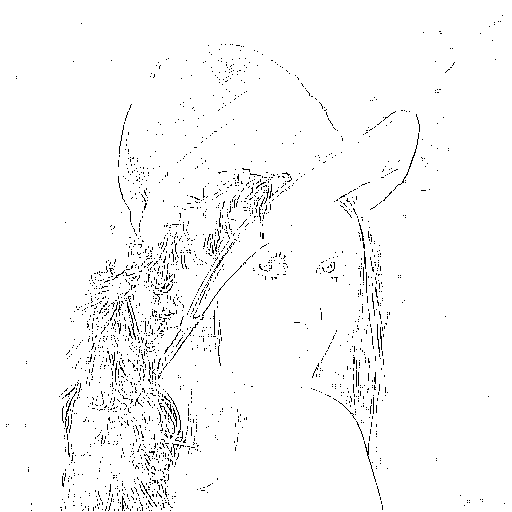
\includegraphics[width=\linewidth]{img/min_var_laplacian.png}
  \caption{Minimum Variance Laplacian with threshold=20}
  \label{fig:min_var_laplacian}
\end{figure}

\subsection{Laplace of Gaussian}
\begin{figure}[H]
  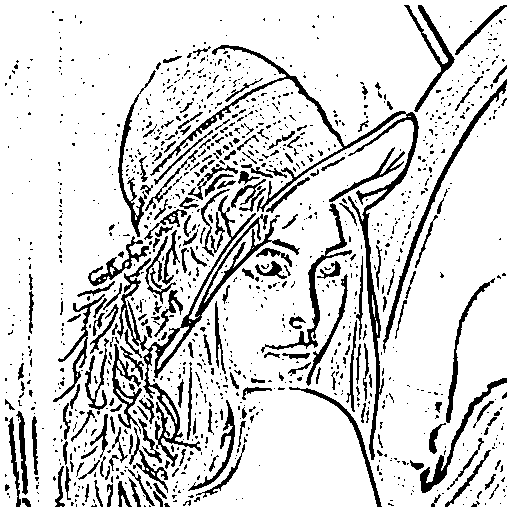
\includegraphics[width=\linewidth]{img/laplacian_of_gaussian.png}
  \caption{Laplace of Gaussian with threshold=3000}
  \label{fig:laplacian_of_gaussian}
\end{figure}

\subsection{Difference of Gaussian}
\begin{figure}[H]
  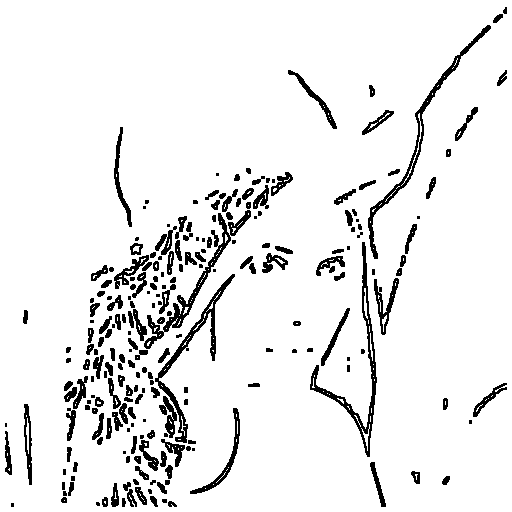
\includegraphics[width=\linewidth]{img/diff_of_gaussian.png}
  \caption{Difference of Gaussian with threshold=1}
  \label{fig:diff_of_gaussian}
\end{figure}

\end{document}
